\subsection{Erstellen des Projektes}
\label{subsec:erstellenProject}
Um die Anwendung zu erstellen, muss der folgende Befehl im Teminal
eingegeben werden:

\begin{zitat}
    dotnet new blazorserver -o MyApp --no-https
\end{zitat}

Dieser Befehl erstellt eine neue Blazor Server Anwendung, mit dem Namen \emph{MyApp} und
konfiguriert die Anwendung ohne das HTTPS-Protokol. Der Name sowie dass kein Https konfiguriert
wird sind optionale Parameter, die nicht mit angegeben werden müssen. Nachdem die Anwendung
erfolgreich installiert wurde, muss die Codezeile \emph{webBuilder.UseUrls("Http://*:5000");
} in der \emph{Program.cs} angegeben werden, um die Anwendung für alle Geräte im LAN verfügbar
ist. Der Code in der \emph{Program.cs} sieht dann folgendermaßen aus:

\begin{lstlisting}[language={[Sharp]C}, caption=Program.cs Code,
    label=lst:programCsCode]
    public class Program
    {
        // Main

        public static IHostBuilder CreateHostBuilder(string[] args) =>
            Host.CreateDefaultBuilder(args)
                .ConfigureWebHostDefaults(webBuilder =>
                {
                    webBuilder.UseStartup<Startup>();
                    webBuilder.UseUrls("Http://*:5000"); // <----
                });
    }
\end{lstlisting}

Mit dem Befehl \emph{dotnet run} kann die Anwendung gestartet werden. Sobald das Programm
gestartet ist, kann mit dem Link \emph{http://<ip>:5000} die Seite erreicht werden. Die
aufgerufene Seite sollte wie folgt angezeigt werden:

\begin{figure}[h]
    \centering
    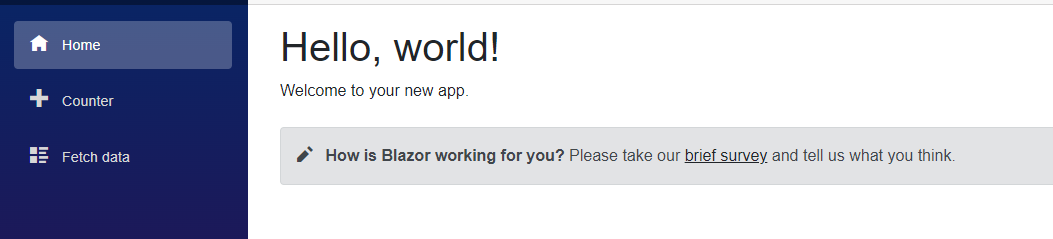
\includegraphics[width=\textwidth, center]{BlazorRasp/ServerTemplate}
    \caption[Blazor Server Template]{Blazor Server Template}
    \label{img:BlazorServerTemplate}
\end{figure}